\section{Setting up EMIO to Allow the Processing System to Control the LEDs}

On a Zedboard, the LEDs can only be controlled via the \gls{pl} (FPGA) side, as the 
physical pins are only connected to the \gls{fpga}. As such, the CPU cannot directly control the LEDs.
Instead, the CPU instructions must be routed through the \gls{pl}, which can be done using the \gls{emio}.

To enable the \gls{emio}:

\begin{enumerate}
    \item Open the Board diagram.
    
        \begin{center}
            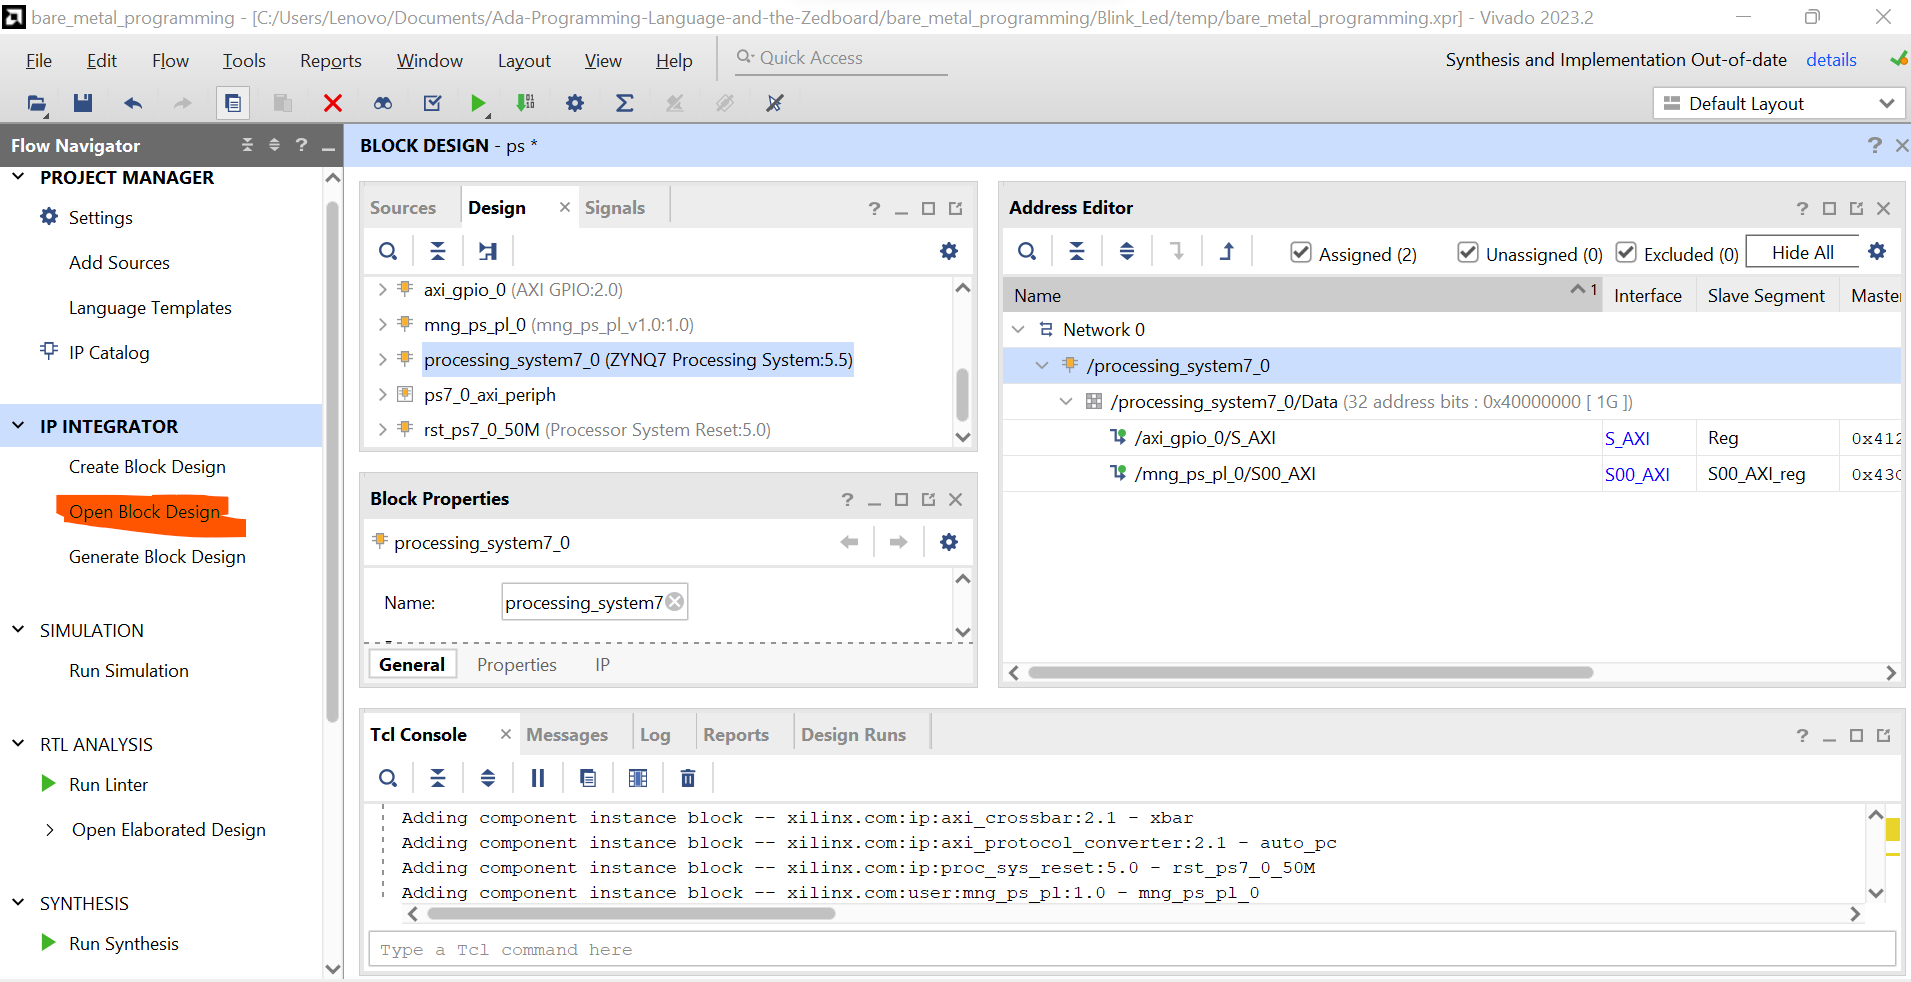
\includegraphics[width=0.9\textwidth]{../Figures/Blink_LED/setup_emio/open_bd.png}
        \end{center}

    \item Double click on the processing system.
    \item Select MIO configuration, I/O Peripherals and at the end open GPIO. Tick EMIO GPIO and in the box select 8.
    
         \begin{center}
            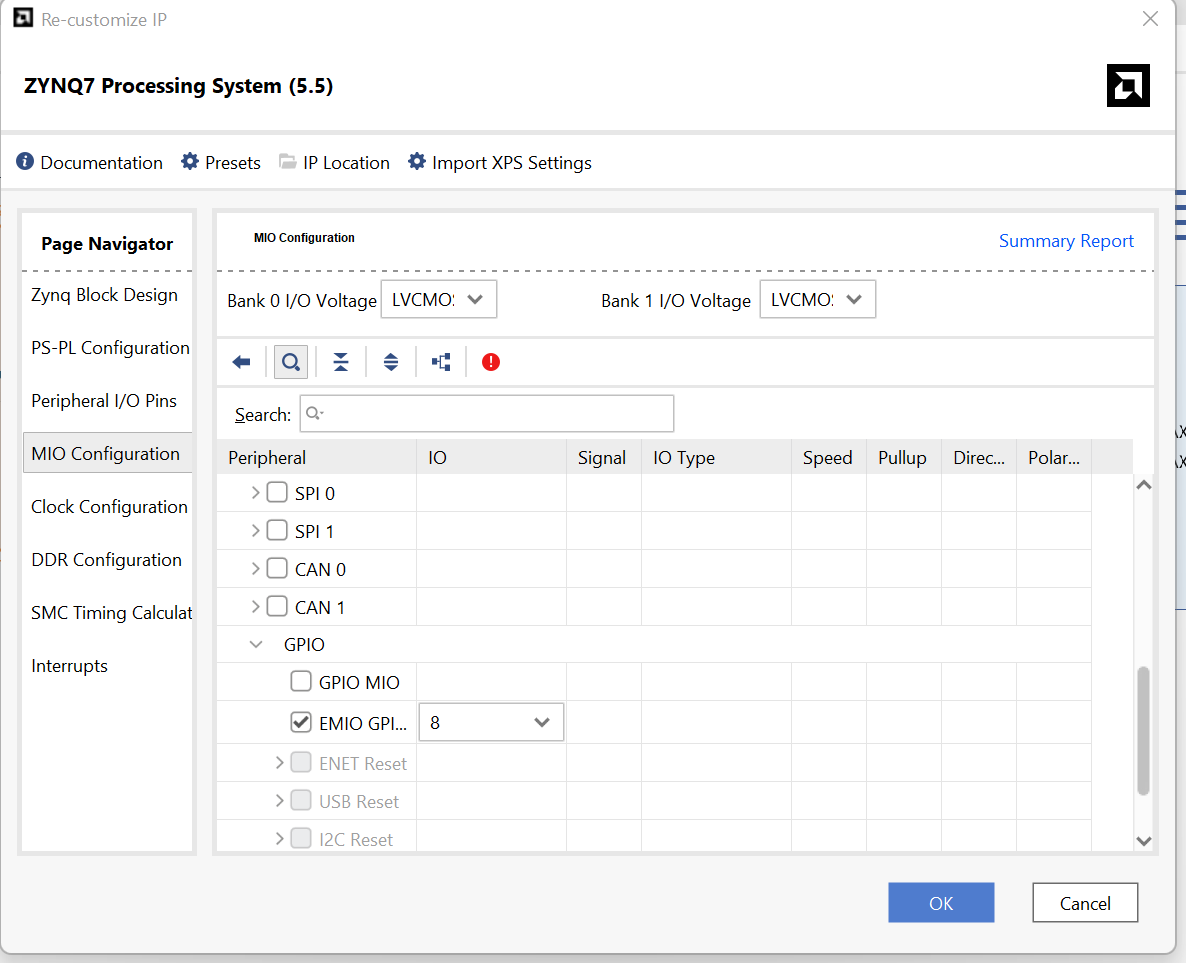
\includegraphics[width=0.9\textwidth]{../Figures/Blink_LED/setup_emio/check_emio.png}
        \end{center}

    \item The \gls{ps} should now have a new port entitled GPIO\_0, with 3 sets of ports each of 8-bits (7:0).
    
        \begin{center}
            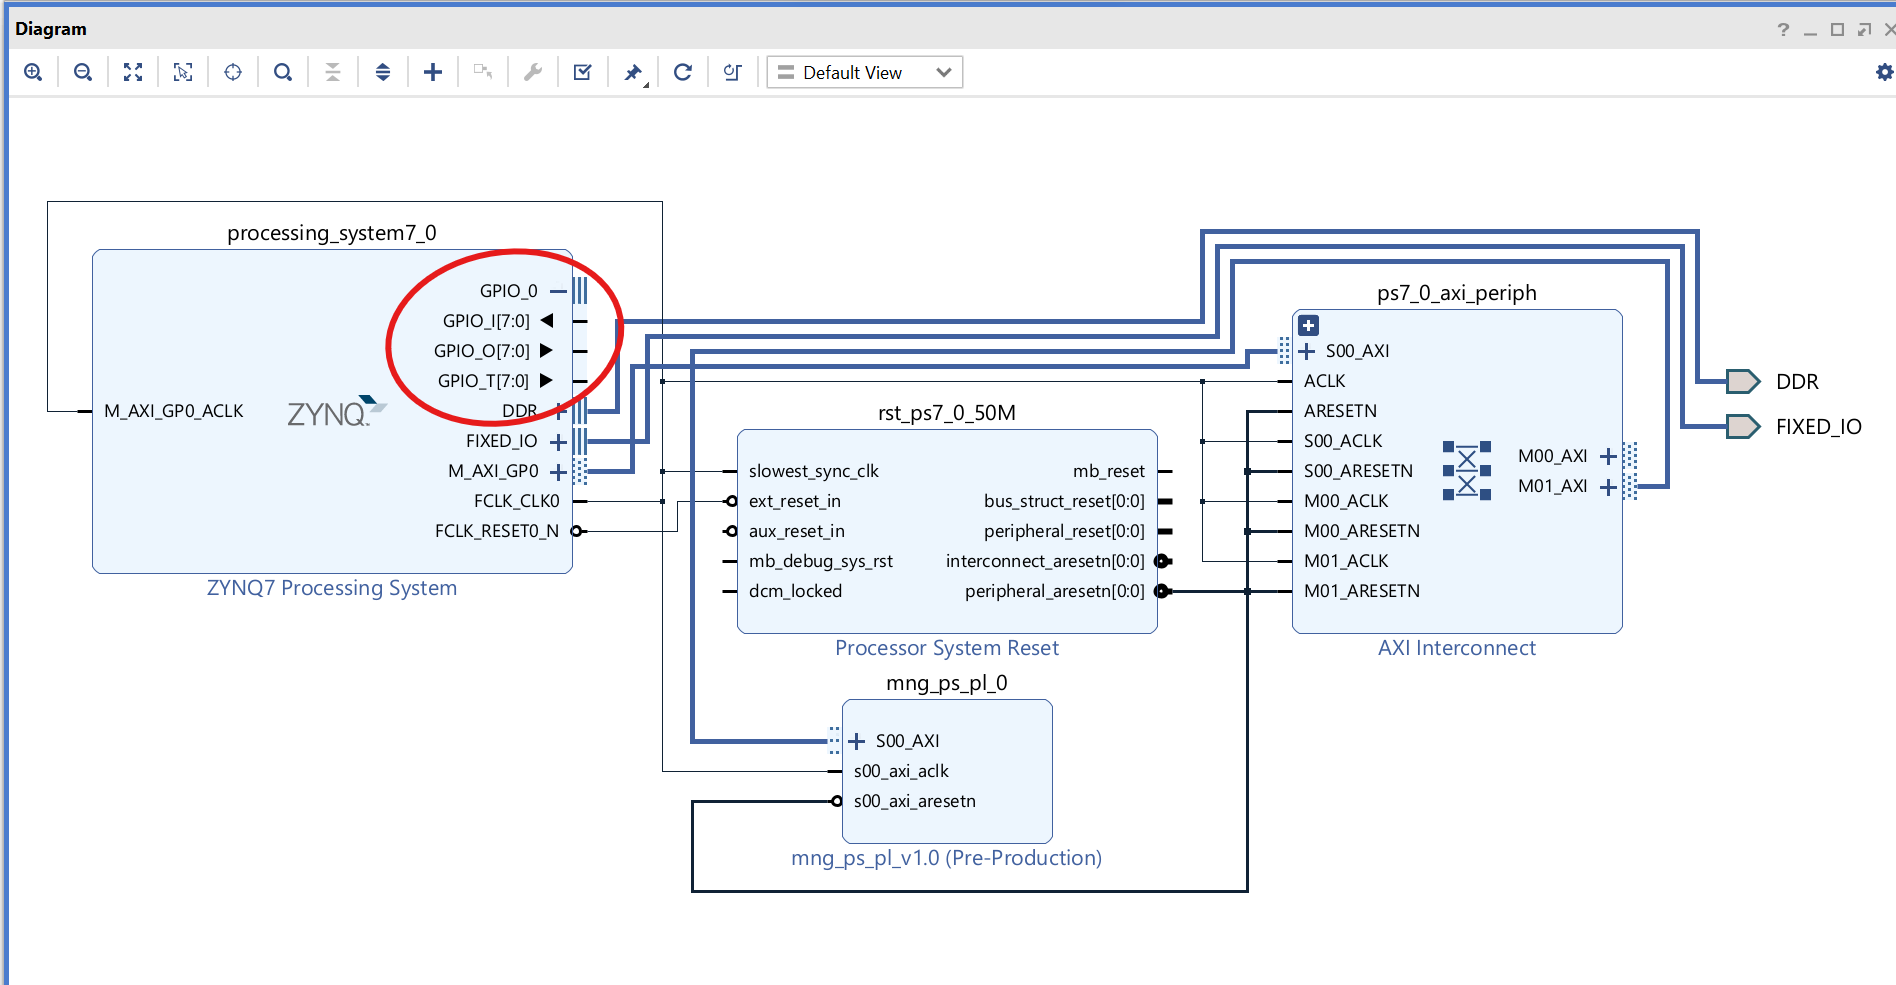
\includegraphics[width=0.9\textwidth]{../Figures/Blink_LED/setup_emio/gpio_0.png}
        \end{center}
    
    \item Right click on GPIO\_0[7:0], and click on "Make External". A port called GPIO\_O\_0[7:0] will be created.
        
        \begin{center}
            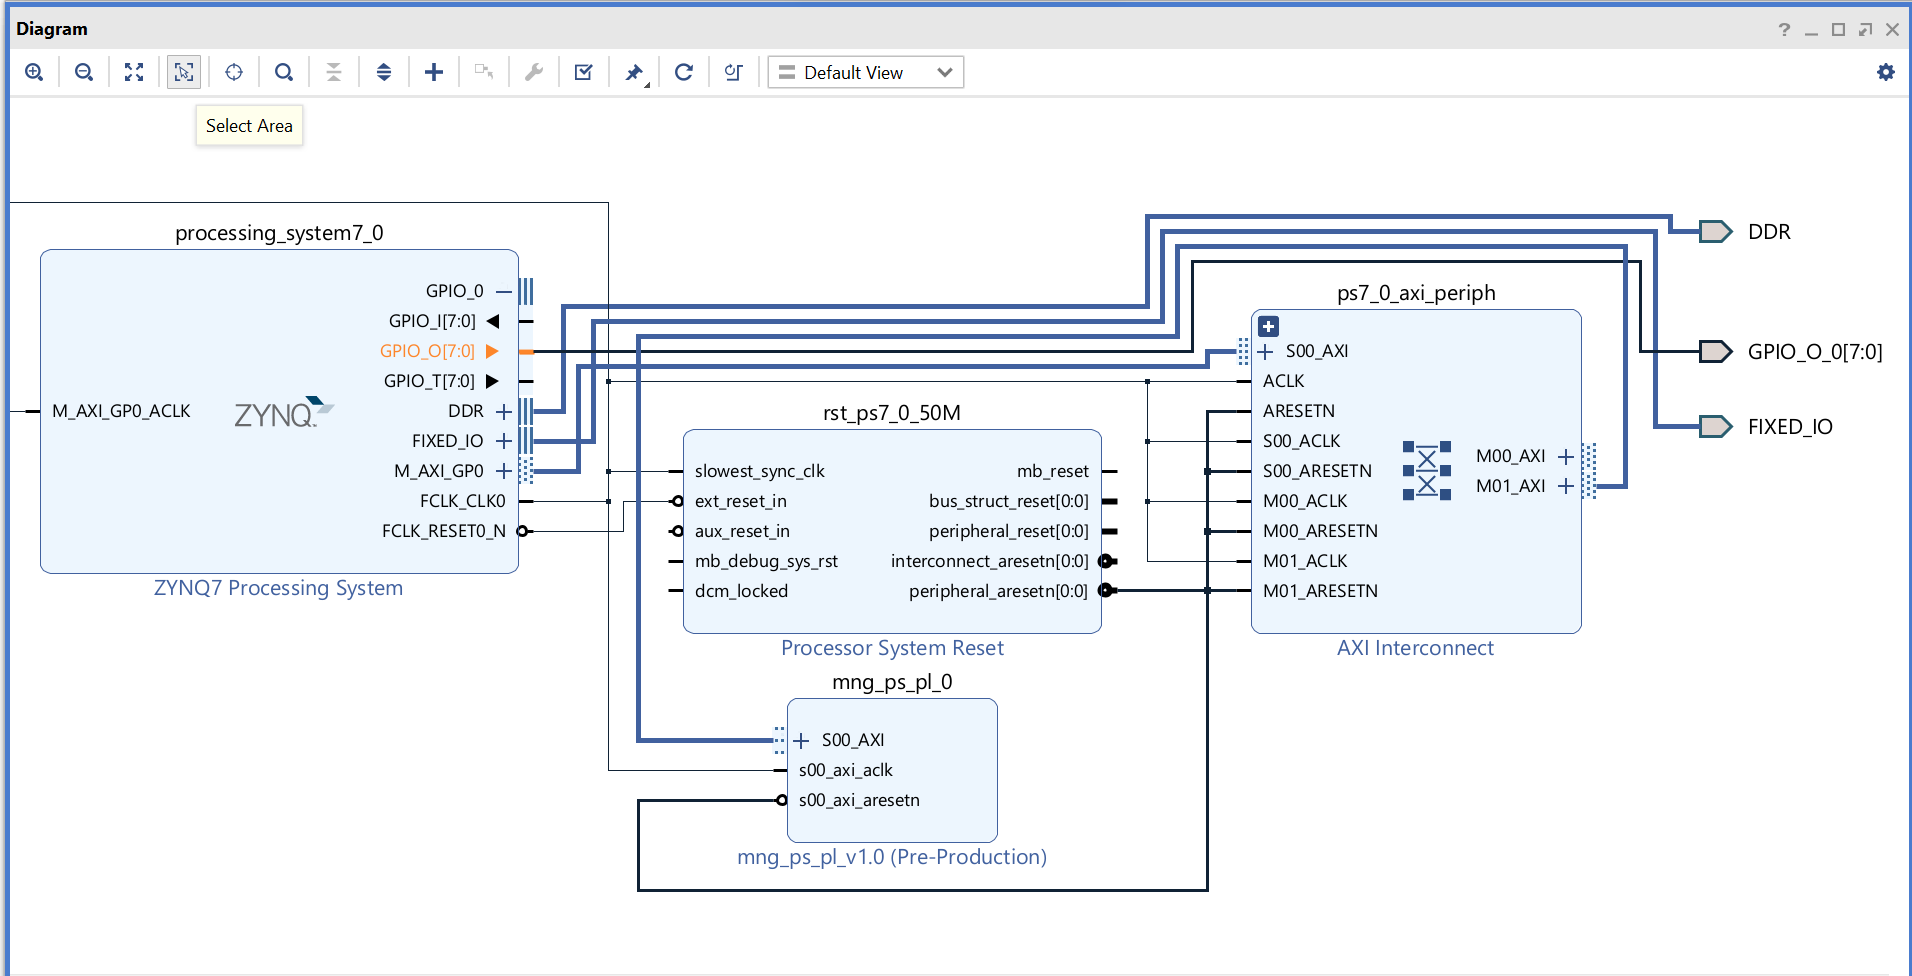
\includegraphics[width=0.9\textwidth]{../Figures/Blink_LED/setup_emio/create_interface_port.png}
        \end{center}

    \item We can rename the port by right clicking it and selecting "External Port Properties". In the box External Port Properties we write the new name.
    
        \begin{center}
            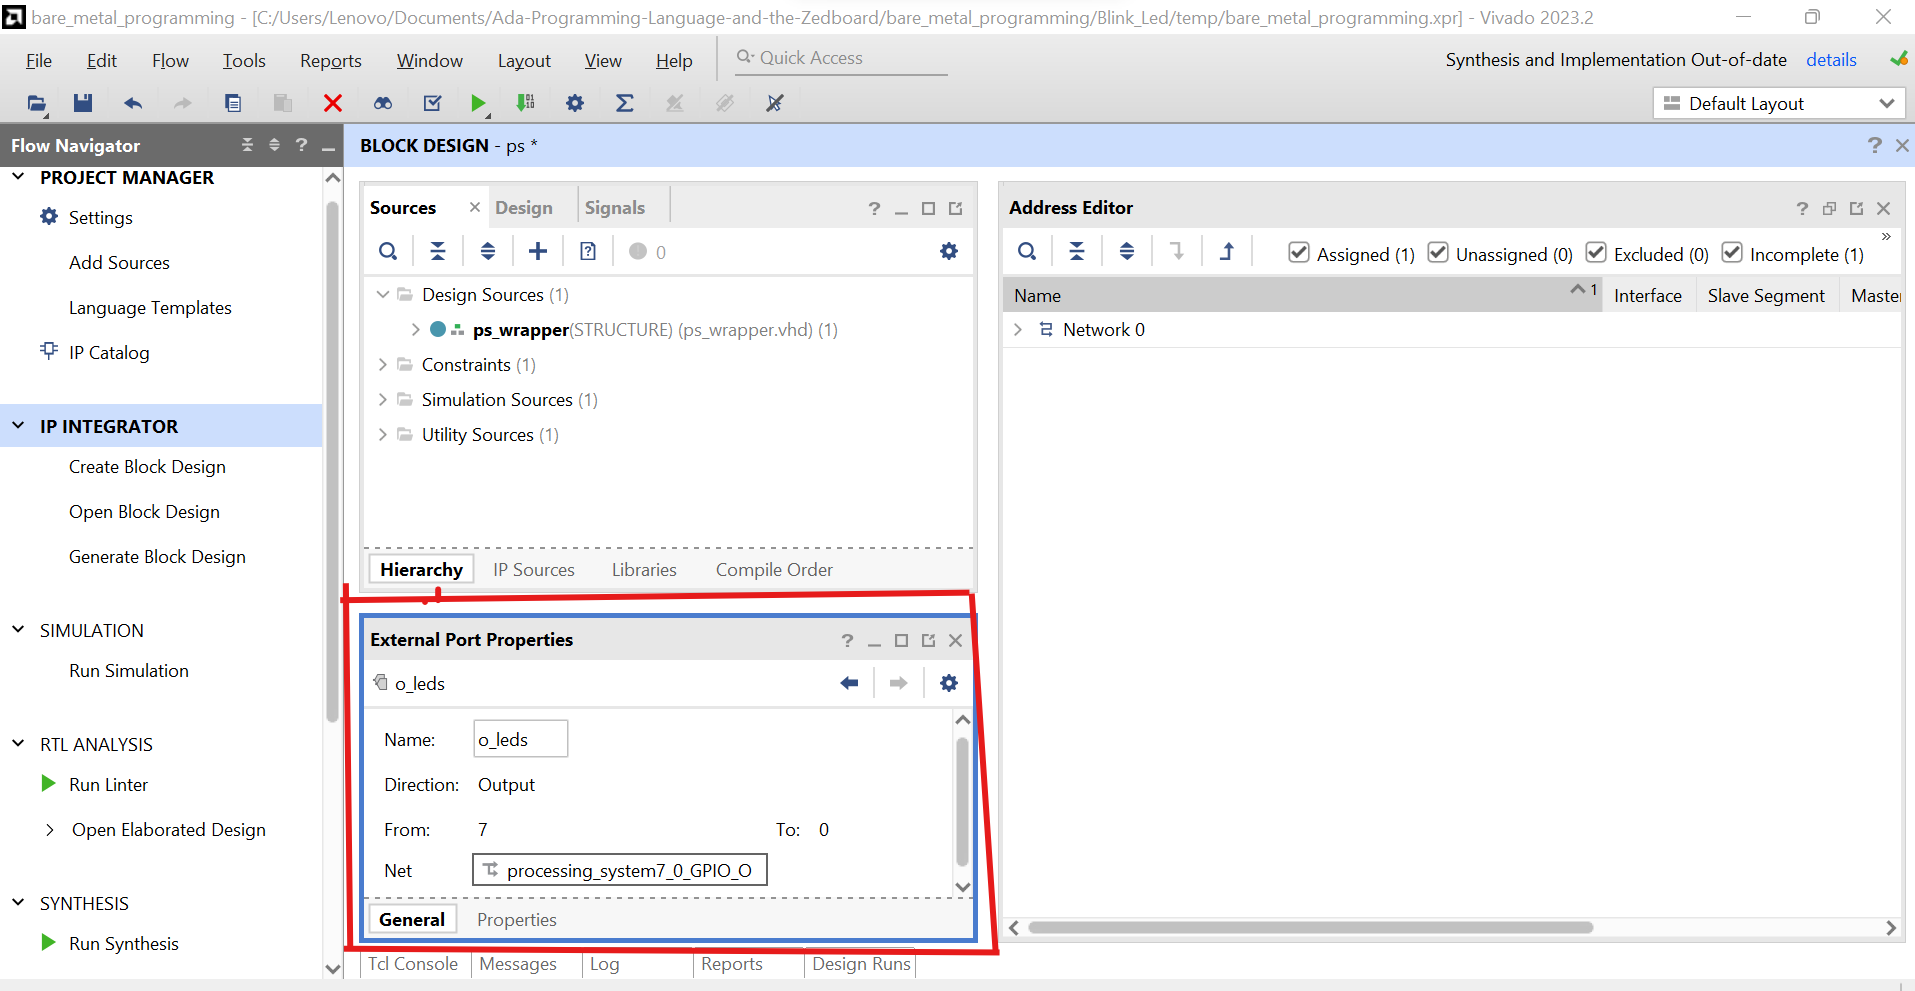
\includegraphics[width=0.9\textwidth]{../Figures/Blink_LED/setup_emio/rename.png}
        \end{center}

    \item The name will now be updated in the board diagram.
    
        \begin{center}
            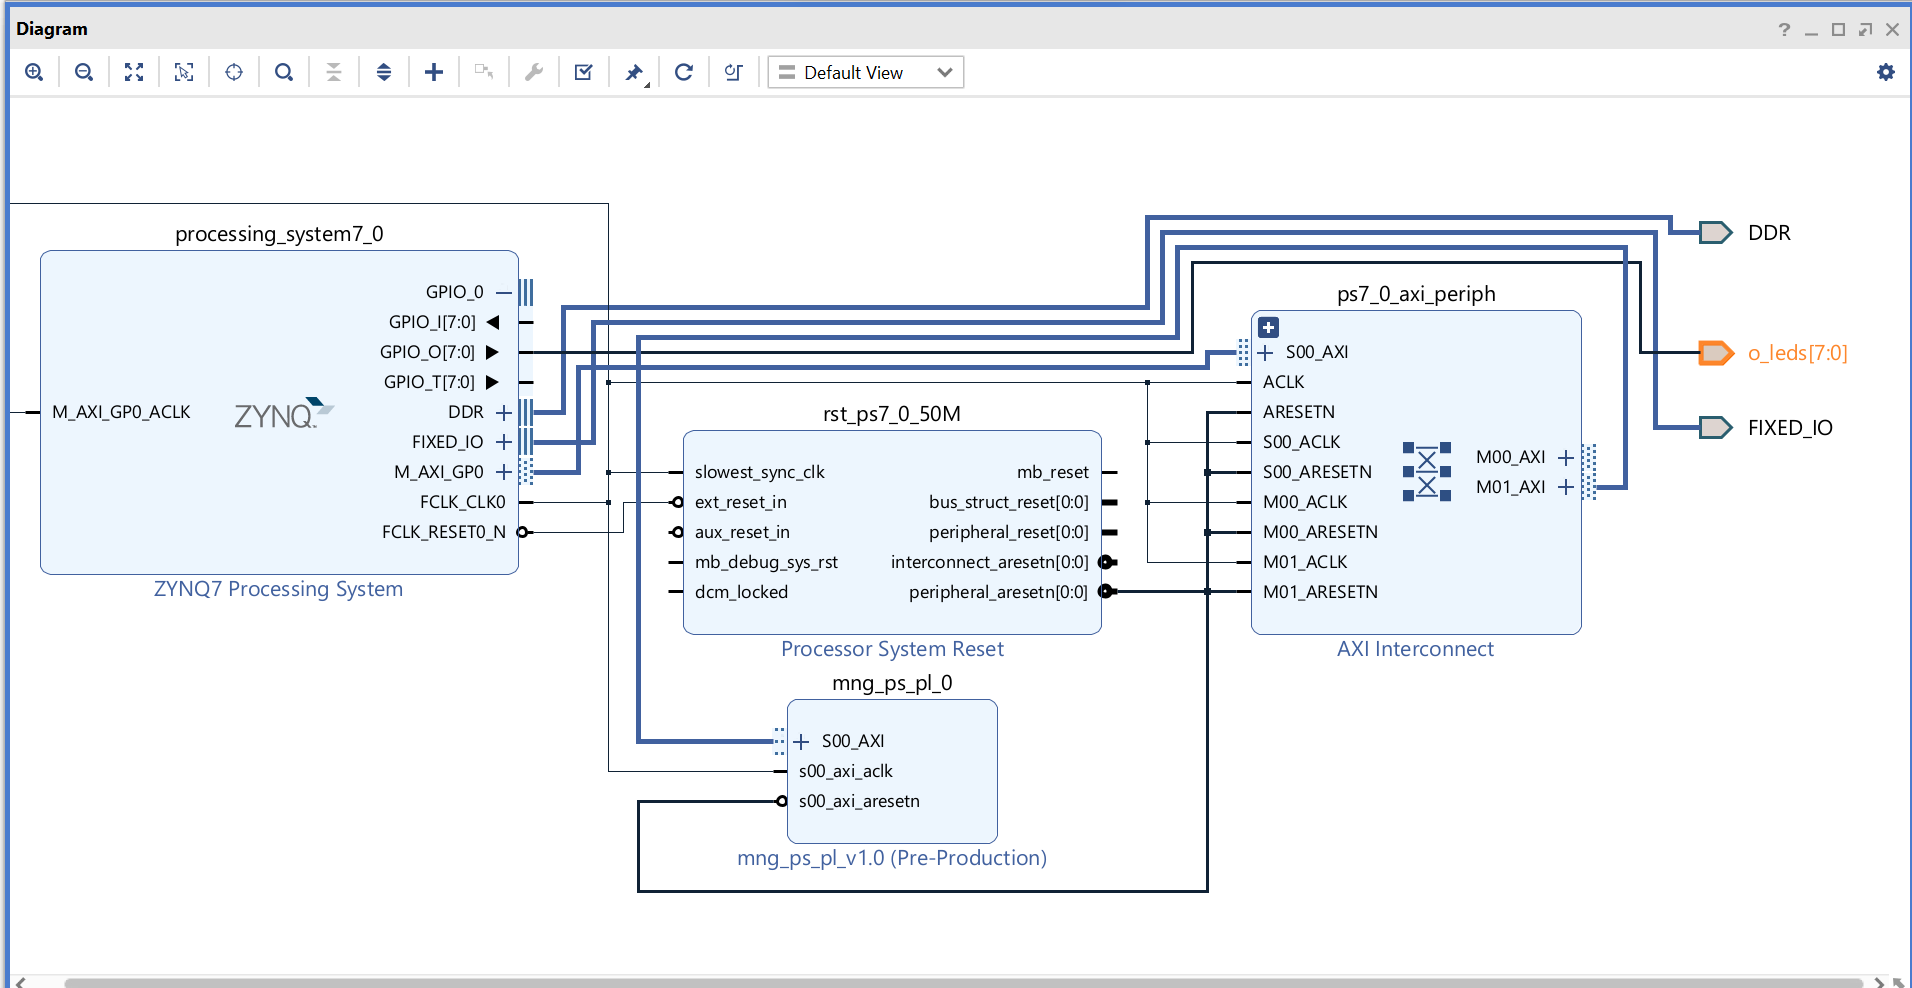
\includegraphics[width=0.9\linewidth]{../Figures/Blink_LED/setup_emio/name_updated.png}
        \end{center}

    \item Inside sources, if not already done, right click on the ps.bd and select generate HDL wrapper. Let Vivado handle updates.
    
        \begin{center}
            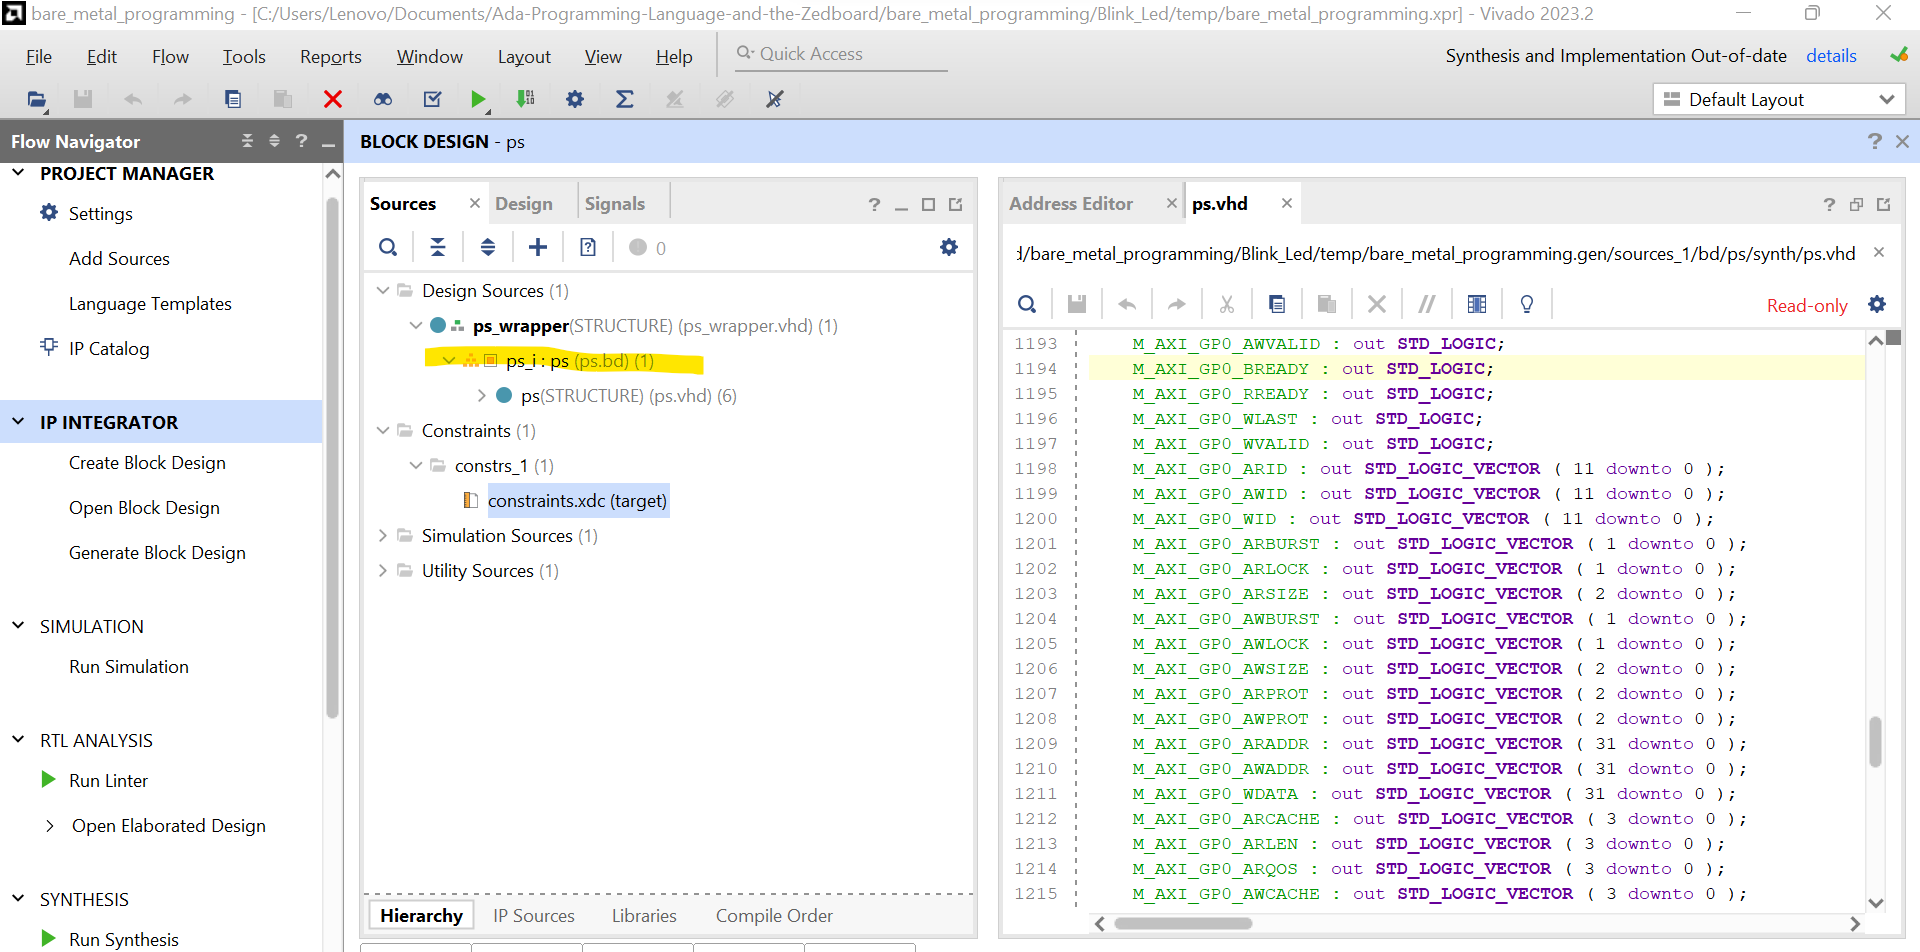
\includegraphics[width=0.9\linewidth]{../Figures/Blink_LED/setup_emio/hdl_wrapper.png}
        \end{center}

\end{enumerate}

    \begin{figure}[H]
        \centering
        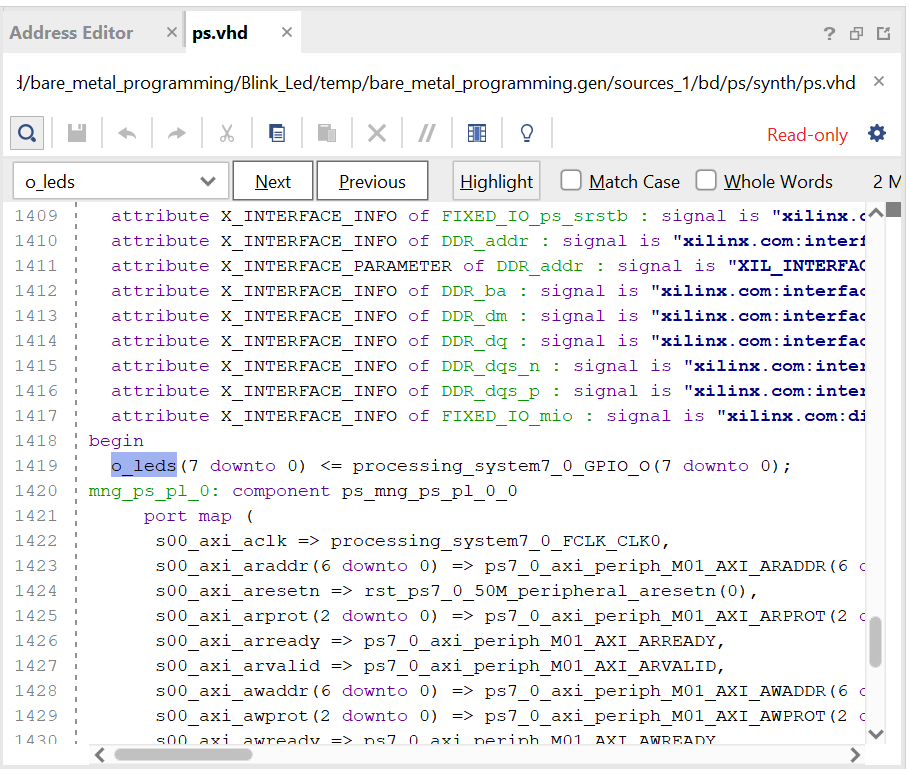
\includegraphics[width=0.9\textwidth]{../Figures/Blink_LED/setup_emio/ps_oleds_connected.png}
        \caption{The \gls{emio} GPIO output from the \gls{ps} is now routed to the \gls{fpga} via o\_leds. }
    \end{figure}


    \begin{figure}[H]
        \centering
        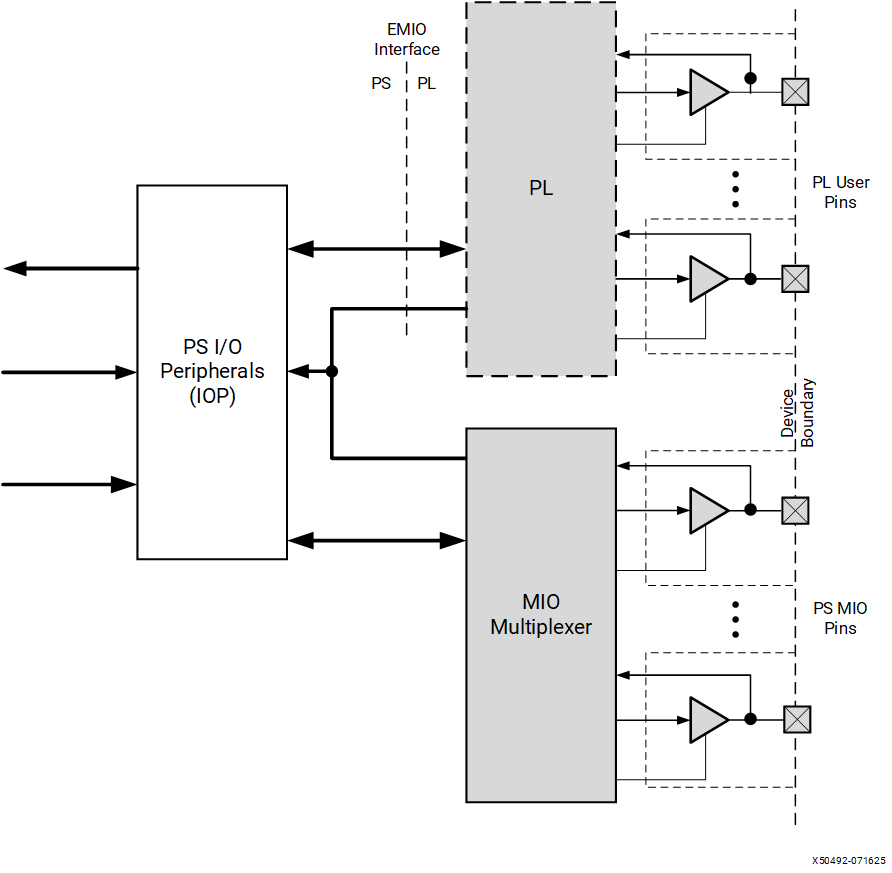
\includegraphics[width=0.9\textwidth]{../Figures/Blink_LED/setup_emio/emio_interface.png}
        \caption{EMIO interface. Taken from UG585 from AMD.}
    \end{figure}

    